\documentclass[12pt]{article}
\usepackage[margin = 1in]{geometry}
\usepackage{graphicx}
\usepackage{caption}
\begin{document}
\begin{Large}
\begin{center}
\textbf{DEFECT DETECTION USING MACHINE VISION}
\end{center}
\end{Large}

\section{Synopsis}
\subsection{Introduction}
\quad Quality checking is an integral step in the production of any product. This involves the maintenance of a desired level of quality in a service or product, by means of attention to every stage of the process of delivery or production.  In manufacturing, quality control is a process that ensures customers receive products free from defects and meet their needs and demands. When done the wrong way, it can put consumers at risk. For example, the recent defect found in Takata airbags resulted in the biggest automotive recall in history$^{[1]}$. Quality makes an important contribution to your company’s reputation, particularly with the growth of social media. Positive reviews and comments can reinforce your own marketing efforts, but also quality problems can have a damaging effect on the companies reputation.\\
\null{\quad}Quality control can help to reduce your production and product support costs. A quality control system helps to lower levels of waste and rework, cutting costs and improving productivity and production efficiency. Delivering quality products can also reduce the number of returns you must handle or the cost of repairing or servicing products in the field. However implementing these techniques using existing technology can be obstructive, ineffective and expensive.\\

{\quad}Thus, our aim is to create a low-cost and an efficient prototype system that is able to detect any defects in an object by using image processing techniques and also estimate the size of such defects.

\subsection{Motivation:}
{\quad}In most of the manufacturing industries, it is common to obtain a few defective products among the perfect ones. On a large scale, it is quite complex to accurately detect a defective product.\\
\null{\quad}Defects in manufacturing occur when a product is improperly manufactured and departs from its intended design. One of the common defects in a product is dimensional inaccuracy. Conventionally, there are two ways to detect these inaccuracies. But the methods employed are usually very expensive, or very slow, or sometimes a combination of both.
\\
\null{\quad}Hence, There is a need for detecting these defects in a cost-effective and efficient manner in the early stages of manufacturing.


\subsection{Problem Statement:}
{\quad}An automated system is to be assembled which can detect and label the dimensional defects of a given object. Such a system must  perform with a high degree of accuracy and also be cost-effective. The designed system must also be easy to operate so that it is deploy-able in a production line with relative ease.

\subsection{Objective:}
{\quad}This work presents a new, real-time, highly automated tool for defect detection based on Image Processing. The specific goals of this investigation are to develop an efficient and non-intrusive dimensional defect detection. These are achieved by creating a machine-vision system able to perform real time acquisition,  image processing and classification. The automatic inspection system will allow the detection and classification of the most frequently occurring dimensional defects in the manufactured products while storing and displaying the possible solutions to the user.


\subsection{Block Diagram:}
\begin{figure}[h]
\centering
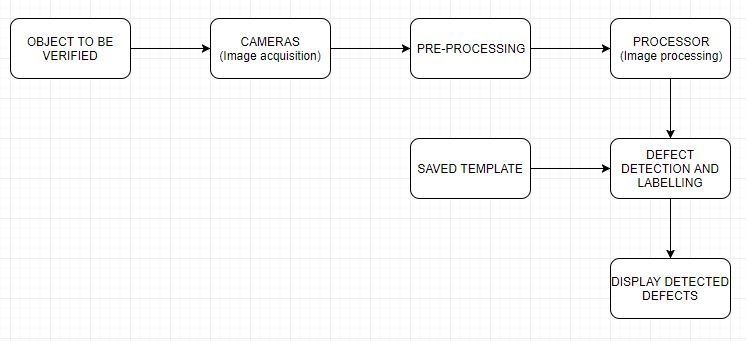
\includegraphics[scale=.8]{bd.jpg}
\caption{Basic Block Diagram}
\end{figure}

A basic block diagram of the proposed project is given above.\\
\null{\quad}The first step is to acquire the image of the object. The image is captured using a camera with the help of a line LASER(3-D triangulation). Since the object can have defects along any axis, we will take multiple images of the object from different angles. Some images are also taken from the top view.\\
\null{\quad}The set of images thus obtained undergo pre-processing, in which the background, noise and other unnecessary parameters are removed from the images.\\
\null{\quad}The pre-processed images undergo image processing using spatial or transform filters. In this stage, the images are compared with another set of images which contains the required result. The difference is detected as a defect. Depending on the type of defect, the object is classified as pass/rework/fail. The size of the defect is also estimated from the given set of images.\\
\null{\quad}Finally the detected defects are marked on the images showing where it is present for further processing.

\subsection{Project Outcome:}
{\quad}The designed automated system will be able to take pictures of the object in all the 3 dimensions using cameras and process the images using image processing techniques. The system will compare the processed image with an initially stored reference image of the same and detect abnormalities or flaws, if any. Finally it will display the area or the part where defect is present and suggest an alternative method for resolving the flaw or problem. 

\subsection{Applications:}
\begin{itemize}
\item{
The proposed system can be used to check defects in manufacturing industries, thus playing a vital role in quality control of the goods manufactured.
}
\item{
If such a system is employed in early stages of production, it can be used to detect the faulty goods beforehand and have a better chance of rectifying the errors, thus reducing wastage.
}
\item{
It can be used in 3D printing and CNC machining to check if there is any defects in the printed materials.
}
\item{
It can be used to check the dimensions of an unknown object.
}

\end{itemize}
\newpage
\section{Literature Survey:}
{\quad}Machine vision (MV) is the technology and methods used to provide imaging-based automatic inspection and analysis for such applications as automatic inspection, process control, and robot guidance, usually in industry. The main task of machine vision systems is providing computer understandable descriptions of objects from either single image or whole array of images. One such area of application  is in automated visual product inspection. An automated visual inspection system must discover and classify possible defects from product images and should be fairly quick and robust. Such an automated system can be assembled with the digital image processing at its core in order to detect defects in large scale manufacturing industries.\\

{\quad}Machine vision system usually finds applications in PCB manufacturing industry since PCBs can be approximated as a 2-D plane. Thus only one image is sufficient to describe a PCB. A study, by Suhasini A.,Sonal D. Kalro, Prathiksha B. G., Meghashree B. S., Phaneendra H. D.$^{[2]}$, utilized a non-contact reference based image processing approach for defect detection and classification and simple image processing algorithm (concerned with arithmetic and logical operation between images where pixel by pixel transformation was applied) for locating the defects on PCB board. A template of defected test PCB image involved many stages which were gray scale image conversion, thresholding, segmentation on basis of different  intensities and were compared with the defect-free PCB images using image subtraction and other procedures. Discrepancies between the images were considered as defects and classified based on similarities and area of occurrence.\\

{\quad}Heriansyah$^{[3]}$ proposed a better technique, which used referential pixel based approach where the PCB could be formed into three groups: the defects on the foreground, on the background and on both. The LVQ neural network had been selected to classify the defects. The designed patterns were trained and tested using the neural network. For the neural network implementation, 2 groups of defects were used for training(i.e., foreground and background). For performance comparison, a pixel  based approach developed which was used to classify seven defects(short, missing hole, pinhole, open, nosebite, spur and etching problem). The stages involved were segmentation, windowing(reference image and detected defects), defects detection, pattern assignment, normalization and classification. All these processes were offline hence did not affect the overall processing time.\\

{\quad}Lins and Givigi$^{[4]}$ had developed a system based machine vision concepts with the goal to automate the crack measurement process. In their method, they have used only a single camera for the processing of the sequence of the images for the crack dimension estimation. The crack model algorithm HSB and RSV were used by which the sequences of the images were subjected to crack detection algorithm in order to detect the crack. The proposed algorithm receives images as and outputs a new image with red particles along the detected crack. The pixel positions of the particles were stored in a vector and passed along to the crack measurement algorithm. With the pixel positions, the algorithm estimates the number of pixels in a cross section and outputs the crack dimension. Li et al$^{[5]}$ have incorporated a new approach for detecting the crack in the defects with the dark color and the low contrast using the fast discrete curvelet waveform and texture analysis. They have initially decomposed and reconstructed the original image using the FDCT algorithm. Then the thresholds of the decomposition coefficients were calculated by the texture feature measurements, from which the surface textures in the images were eliminated. Finally, by extracting the contours from the reconstructed images, the expected image without texture but with crack defect contours was obtained.\\

{\quad}But these systems works well for a 2-D view since we are taking an image or a set of images. These methods fail to work for 3-D objects. M Jonathan Wu Etal$^{[6]}$ designed a 3-D sensing system applying artificial intelligence methodology for quantity assurance in automatic manufacturing processes. Using a single 2-D CCD camera, laser structured light and fuzzy techniques for rule based decision-making, it was possible to successfully interpret 3-D view. The surface environment information was converted into the orientation,curvature and depth of the shape to incorporate into symbolic 3-D object oriented information base and reasoning algorithm.\\




\subsection{Mathematical Analysis:}
{\quad}In order for a object to be scanned so that the defects can be detected, a simple 3-D triangulation setup is created using a line LASER and a camera.\\

{\quad}The image above shows a very simple triangulation setup using a camera and a line LASER. The LASER diode is positioned such that it creates a triangle with the view direction of the camera. As you can see from the image, the LASER line projects on the object and intersects the view direction of the camera exactly at the axis of rotation of the object. The angle at the intersection of the LASER line and the view direction (THETA) provides us with the first tool for extracting depth related information from the image captured by the camera.
\begin{figure}
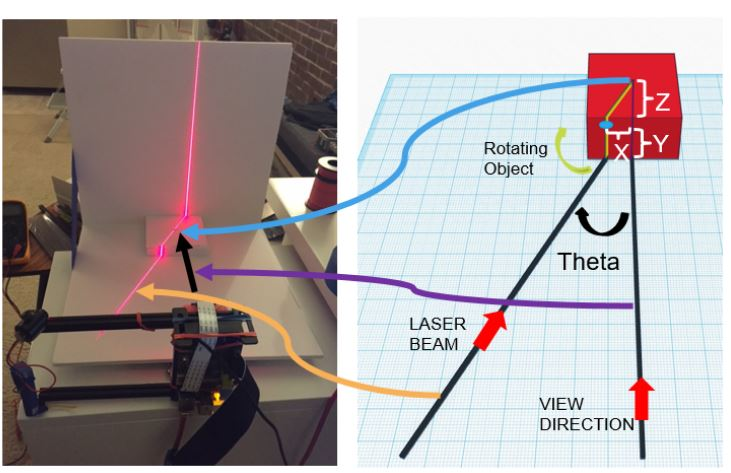
\includegraphics[scale=1]{lasercamera.jpg}
\caption{A simple triangulation setup consisting of a Line LASER diode projecting a line on the 3D object}
\end{figure}\\

{\quad}The length of X and Y can be obtained from the image itself.
$$X=N_v * X_s$$
$$Y=Scanline * Y_s$$
where,\\
$N_v$ is the number of pixels from view direction\\
$X_s$ is X scaling factor\\
and,$Y_s$ is Y scaling factor\\
\begin{figure}[h]
\centering
\begin{minipage}{.5\textwidth}
  \centering
  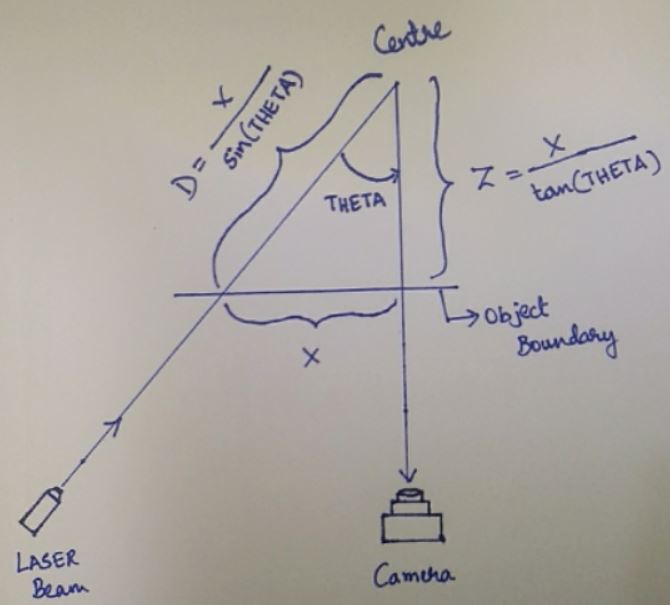
\includegraphics[scale=.5]{triangle.jpg}
  \captionof{figure}{Top view of the triangulation setup}
  %\label{fig:test1}
\end{minipage}%
\begin{minipage}{.5\textwidth}
  \centering
  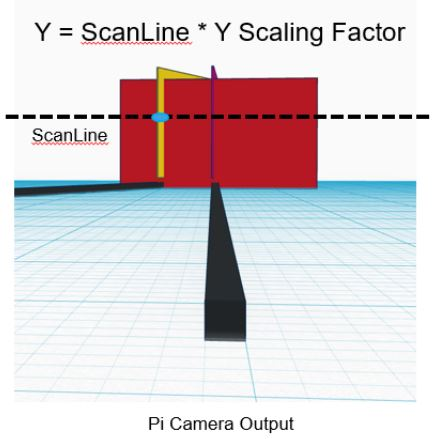
\includegraphics[scale=.7]{yline.jpg}
  \captionof{figure}{View from the camera}
  %\label{fig:test2}
\end{minipage}
\end{figure}
{\quad}Since we know the angle(THETA), we can calculate the depth of the image or the Z component as,
$$Z=\frac{X}{\tan(THETA)}$$
$$D=\frac{X}{\sin(THETA)}$$

{\quad}Let the set of images of the object on which the LASER is incident be defined as,\\
\begin{center}
$f_i(x,y),{\quad}0{\leq}i<N${\quad}(N is the number of images taken)
\end{center}

{\quad}Let the set of images of the object which does not have the LASER incident on it be defined as,\\
\begin{center}
$g_i(x,y),{\quad}0{\leq}i<N$
\end{center}

{\quad} Initially the backgrounds of all the images are removed by subtracting the background image from the set of images present. If $b(x,y)$ is an image only containing the background, then,
$$f'_i(x,y)=f_i(x,y)-b(x,y),{\quad}\forall i\in[0,N)$$
The images now contain only the object devoid of the background. After removing the background it checks for any defects by comparing $f'_i(x,y)$ with respect to a previously stored images of a perfectly fine, LASER incident object. The comparison is done using subtraction or bit-wise XOR operation,
$$f_i"(x,y)=f'_i(x,y)-p_i(x,y),{\quad}\forall i\in[0,N)$$
or,
$$f_i"(x,y)=f'_i(x,y){\wedge}p_i(x,y),{\quad}\forall i\in[0,N)$$
where, $p_i(x,y)$ is a set of images of an object without any defects, stored within the processor.\\

{\quad}The resultant image $f"_i(x,y)$ contains a contour which basically is the deviation from the required value. This represents the defect present in the object. The size of the defect is later estimated by comparing all such images which do not match with $p_i(x,y)$. If $f"_i(x,y)$ does not have any contours, then it can be classified as an object with no defects.\\

{\quad}Finally, the contour is superimposed on the corresponding $g_i(x,y)$ to mark where the defect is present. Hence the set of output images is,
$$h_i(x,y)=f_i"(x,y)\vert g_i(x,y)$$

\subsection{Software Requirements:}
\subsubsection{OpenCV:}
{\quad}OpenCV (Open Source Computer Vision) is a library of programming functions mainly aimed at real-time computer vision. It was originally developed by Intel and is released under BSD license. Hence it is free for both academic and commercial purposes.  It has C++, C, Python and Java interfaces and supports Windows, Linux, Mac OS, iOS and Android. OpenCV was designed for computational efficiency and with a strong focus on real-time applications. Written in optimized C/C++, the library can take advantage of multi-core processing. Enabled with OpenCL, it can take advantage of the hardware acceleration of the underlying heterogeneous compute platform.

\subsubsection{Arduino IDE:}
{\quad}The Arduino project provides the Arduino integrated development environment (IDE), which is a cross-platform application written in the programming language Java. It originated from the IDE for the languages Processing and Wiring. It includes a code editor with features such as text cutting and pasting, searching and replacing text, automatic indenting, brace matching, and syntax highlighting, and provides simple one-click mechanisms to compile and upload programs to an Arduino board. It also contains a message area, a text console, a toolbar with buttons for common functions and a hierarchy of operation menus.\\

{\quad}The Arduino IDE supports the languages C and C++ using special rules of code structuring. The Arduino IDE supplies a software library from the Wiring project, which provides many common input and output procedures. User-written code only requires two basic functions, for starting the sketch and the main program loop, that are compiled and linked with a program stub main() into an executable cyclic executive program with the GNU tool-chain, also included with the IDE distribution. The Arduino IDE employs the program avrdude to convert the executable code into a text file in hexadecimal encoding that is loaded into the Arduino board by a loader program in the board's firmware.

\subsubsection{Python:}
{\quad}Python is a widely used high-level programming language for general-purpose programming.Python has a design philosophy that emphasizes code readability and a syntax that allows programmers to express concepts in fewer lines of code than might be used in languages such as C++ or Java.The language provides constructs intended to enable writing clear programs on both a small and large scale.Python features a dynamic type system and automatic memory management and supports multiple programming paradigms, including object-oriented, imperative, functional programming, and procedural styles. Python can be run on variety of OS like Windows, macOS, Linux and even Raspbian.


\subsection{Hardware Requirements:}
\subsubsection{Arduino Uno:}
{\quad}The Arduino Uno is a micro-controller board based on the ATmega328 (data-sheet). It has 14 digital input/output pins (of which 6 can be used as PWM outputs), 6 analog inputs, a 16 MHz crystal oscillator, a USB connection, a power jack, an ICSP header, and a reset button. It contains everything needed to support the micro-controller; simply connect it to a computer with a USB cable or power it with a AC-to-DC adapter or battery to get started.
The Uno differs from all preceding boards in that it does not use the FTDI USB-to-serial driver chip. Instead, it features the Atmega16U2 (Atmega8U2 up to version R2) programmed as a USB-to-serial converter.

\subsubsection{Raspberry Pi:}
{\quad}Raspberry Pi is an ARM based credit card sized SBC(Single Board Computer) created by Raspberry Pi Foundation. Raspberry Pi runs Debian based GNU/Linux operating system Raspbian and ports of many other OSes exist for this SBC.
The Raspberry Pi 3 Model B is the third generation Raspberry Pi. This powerful credit-card sized single board computer can be used for many applications and supersedes the original Raspberry Pi Model B+ and Raspberry Pi 2 Model B.
Additionally it adds wireless LAN and Bluetooth connectivity making it the ideal solution for powerful connected designs.

\subsubsection{Camera module:}
{\quad}The Raspberry Pi camera module can be used to take high-definition video, as well as stills photographs. The camera consists of a small (25mm by 20mm by 9mm) circuit board, which connects to the Raspberry Pi's Camera Serial Interface (CSI) bus connector via a flexible ribbon cable. The camera's image sensor has a native resolution of five megapixels and has a fixed focus lens. The software for the camera supports full resolution still images up to 2592x1944 and video resolutions of 1080p30, 720p60 and 640x480p60/90.
\newpage

\section{References}
\begin{enumerate}
\item{Consumer Reports. (July 14,2017). \emph{Takata Airbag Recall - Everything You Need to Know}, retrieved on September 20,2017.\\
URL: https://www.consumerreports.org/cro/news/2016/05/everything-you-need-to-know-about-the-takata-air-bag-recall/index.htm}
\item{
Suhasini A.,Sonal D. Kalro, Prathiksha B. G., Meghashree B. S., Phaneendra H. D., \emph{PCB Defect Detection Using Image Subtraction Algorithm}, International Journal of Computer Science Trends and Technology (IJCST) – Volume 3 Issue 3, May-June 2015.
}
\item{R. Heriansyah and S. A. R. Abu-Bakar(2004), \emph{Defects classification on bare PCB using multiple learning vector quantization neural network paradigm}, International Conference on Computer Graphics, Imaging, and Visualization 2004 (CGIV 2004), pp.50-53.}
\item{
Romulo Gonçalves Lins, Sidney N. Givigi, \emph{Automatic crack detection and
measurement based on image analysis}, IEEE Trans. Instrum. Meas., 65 (3) (2016), pp. 583-590}
\item{Xueqin Li, Honghai Jiang, Guofu Yin, \emph{Detection of surface crack defects on ferrite magnetic tile}, NDT E Int., 62 (2014), pp. 6-13}
\item{Q.M. Jonathan Wu, M.F. Ricky Lee and Clarence W. de Silva,
\emph{Intelligent 3-D Sensing in Automated Manufacturing Processes}, IEEE, pp. 334-339, 2001.}
\item{Makerzone. (July 12,2016). \emph{Raspberry Pi + MATLAB based 3D Scanner}, retrieved on September 15,2017\\
URL: https://makerzone.mathworks.com/resources/raspberry-pi-matlab-based-3d-scanner/}
\end{enumerate}

\end{document}
